\chapter{Needs}
This chapter contains the operational needs necessary to solve the problems described in the previous chapter. 



\begin{enumerate}
\item[•] It shall be possible for the different users of the system to communicate via the system. 
\item[•] The system shall provide the users with real time static and dynamic information. 
\item[•] The system shall be able to track the geographical position of the users of the system. 
\item[•] The system shall provide the users of the system with the geographical position data of the users of the system. 
\end{enumerate}




\begin{figure}[H]
\centering
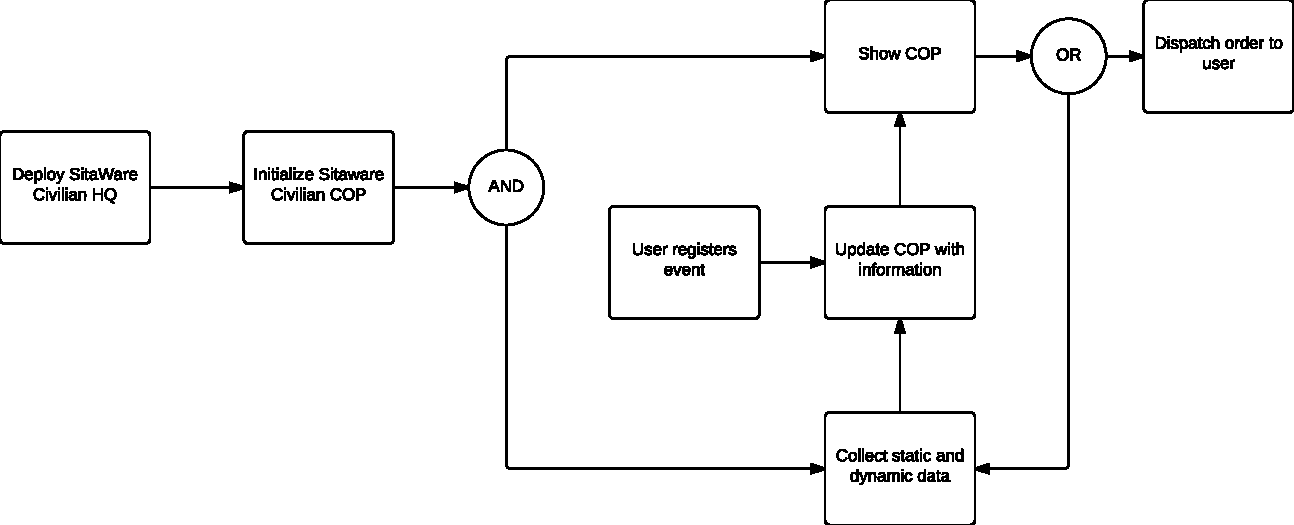
\includegraphics[width=0.95\textwidth]
{billeder/functional_flow_block_diagram.pdf}
\caption{Functional flow block diagram.}
\label{fig:functional_flow_block_diagram}
\end{figure}